\documentclass[fleqn, 11pt]{beamer}
\usepackage[spanish]{babel}
\usepackage[utf8]{inputenc}
\usepackage{amsmath, amssymb, amsfonts}
\usepackage{parskip}
\usepackage[left = 18mm, right = 18mm, bottom = 18mm, top = 18mm]{geometry}
\usepackage{tcolorbox}
\tcbuselibrary{theorems}
\tcbuselibrary{breakable}
\usepackage{colortbl}
\usepackage{array, tabularx}
\usepackage[pdftex, hidelinks]{hyperref}
\usepackage{multirow}
\usepackage{multicol}
\usepackage{enumerate}
\usepackage{graphicx}

\usepackage[proportional,scaled=1.064]{erewhon}
\usepackage[erewhon,vvarbb,bigdelims]{newtxmath}
\usepackage[T1]{fontenc}
\renewcommand*\oldstylenums[1]{\textosf{#1}}

\renewcommand{\labelenumi}{\textit{\roman{enumi}.}}
\newcommand{\gradial}{\hspace{0.9mm} 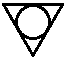
\includegraphics[width = 3mm]{gradial.png} \hspace{1mm}}

\tcbsetforeverylayer{autoparskip}

\tcbset{theorem full label supplement={hypertarget={#1}}}

\newtcbtheorem[auto counter, number freestyle = {\noexpand \arabic{\tcbcounter}}]{definicion}{D\hspace{0.1mm}e\hspace{0.1mm}f\hspace{0.4mm}i\hspace{0.1mm}n\hspace{0.1mm}i\hspace{0.1mm}c\hspace{0.1mm}i\hspace{0.1mm}ó\hspace{0.1mm}n}{colback = white, colframe = black, fonttitle = \bfseries}{def}

\newtcbtheorem[auto counter, number freestyle = {\noexpand \arabic{\tcbcounter}}]{teorema}{T\hspace{0.1mm}e\hspace{0.1mm}o\hspace{0.1mm}r\hspace{0.1mm}e\hspace{0.1mm}m\hspace{0.1mm}a}{colback = white, colframe = black, fonttitle = \bfseries}{teo}

\newtcbtheorem[use counter from = teorema]{proposicion}{P\hspace{0.1mm}r\hspace{0.1mm}o\hspace{0.1mm}p\hspace{0.1mm}o\hspace{0.1mm}s\hspace{0.1mm}i\hspace{0.1mm}c\hspace{0.1mm}i\hspace{0.1mm}ó\hspace{0.1mm}n}{colback = white, colframe = black, fonttitle = \bfseries}{prop}

\newtcbtheorem[use counter from = teorema]{corolario}{C\hspace{0.1mm}o\hspace{0.1mm}r\hspace{0.1mm}o\hspace{0.1mm}l\hspace{0.1mm}a\hspace{0.1mm}r\hspace{0.1mm}i\hspace{0.1mm}o}{colback = white, colframe = black, fonttitle = \bfseries}{cor}

\newtcbtheorem[use counter from = teorema]{lema}{L\hspace{0.1mm}e\hspace{0.1mm}m\hspace{0.1mm}a}{colback = white, colframe = black, fonttitle = \bfseries}{lem}

\newtcbtheorem[auto counter, number freestyle = {\noexpand \arabic{\tcbcounter}}]{ejemplo}{E\hspace{0.1mm}j\hspace{0.1mm}e\hspace{0.1mm}m\hspace{0.1mm}p\hspace{0.1mm}l\hspace{0.1mm}o}{colback = white, colframe = black, fonttitle = \bfseries}{ejem}

\begin{document}
    %Portada
    \begin{titlepage}
        \centering
        \phantom{.}

        {\Huge \textbf{Universidad Autónoma del Estado de México}\par}
        \vspace{0.6cm}

        {\Huge \textbf{Facultad de Ciencias}\par}
        \vspace{0.6cm}

        {\Huge \textbf{Licenciatura en Matemáticas}\par}
        \vspace{1.2cm}

        {\Huge \textbf{Teoría de gráficas}\par}
        \vspace{1.1cm}

        {\Huge \textbf{Trabajo de investigación:}\par}

        {\huge \textbf{Gráfica Gradial}\par}
        \vspace{0.6cm}

        {\huge \textbf{Profesora:}\par}
        \vspace{0.3cm}
        {\huge \textsl{Berta Zavala Santana}}\par
        \vspace{0.6cm}

        {\huge \textbf{Alumno:}\par}
        \vspace{0.3cm}
        {\huge \textsl{Osmar Dominique Santana Reyes}}\par
        \vspace{1.2cm}

        {\huge \textbf{Semestre: 2023B}\par}

        \vspace{1.8cm}
        \raggedleft{\LARGE Fecha de Entrega: 4 de diciembre de 2023}\par         %Alinear a la derecha
    \end{titlepage}

    \begin{definicion}[beforeafter skip = 4mm]{}{grafica_de_gradial}
        Sean $ G_1 $ y $ G_2 $ gráficas tales que $ \textnormal{V}(G_1) \cap \textnormal{V}(G_2) = \emptyset $. Se define a $ G_1 \gradial G_2 = (\textnormal{V}, \textnormal{A}) $ como la \textbf{gráfica gradial de $ G_1 $ y $ G_2 $} con \vspace{2mm}
        
        $ \textnormal{V}(G_1 \gradial G_2) = \textnormal{V}(G_1) \cup \textnormal{V}(G_2) $ \quad y \vspace{-1mm}
        \begin{align*}
            \hspace{-9mm} \textnormal{A}(G_1 \gradial G_2) =& \bigl\{ uv \mid u \in \textnormal{V}(G_1), \, v \in \textnormal{V}(G_2), \textnormal{ gr}_{G_1}(u) + \textnormal{gr}_{G_2}(v) = \delta(G_1) + \Delta(G_2) \bigr\} \, \cup \\
            & \bigl\{ uv \mid u \in \textnormal{V}(G_2), \, v \in \textnormal{V}(G_1), \textnormal{ gr}_{G_2}(u) + \textnormal{gr}_{G_1}(v) = \delta(G_2) + \Delta(G_1) \bigr\}
        \end{align*}
    \end{definicion}

    En términos de la definicion anterior, para hallar las aristas de la gráfica gradial, es necesario resolver las siguientes ecuaciones diofantinas:

    $ \textnormal{gr}_{G_1}(u) + \textnormal{gr}_{G_2}(v) = \delta(G_1) + \Delta(G_2) $ \; y \; $ \textnormal{gr}_{G_2}(u') + \textnormal{gr}_{G_1}(v') = \delta(G_2) + \Delta(G_1) $

    donde $ u, v' \in \textnormal{V}(G_1) $ \, y \, $ v, u' \in \textnormal{V}(G_2) $. Algunas soluciones particulares para cada ecuación son: \\
    $ \textnormal{gr}_{G_1}(u) = \delta(G_1) $, $ \textnormal{gr}_{G_2}(v) = \Delta(G_2) $, $ \textnormal{gr}_{G_2}(u') = \delta(G_2) $ \, y \, $ \textnormal{gr}_{G_1}(v') = \Delta(G_1) $.

    De esta manera, las soluciones para cada ecuación son:

    $ \textnormal{gr}_{G_1}(u) = \delta(G_1) + l, \textnormal{gr}_{G_2}(v) = \Delta(G_1) - l, $ con $ l = 0,1, \ldots, \max\left\lbrace \Delta(G_1) - \delta(G_1), \Delta(G_2) \right\rbrace $ \, y 
    
    $ \textnormal{gr}_{G_2}(u') = \delta(G_2) + l, \textnormal{gr}_{G_1}(v') = \Delta(G_1) - l, $ con $ l = 0,1, \ldots, \max\left\lbrace \Delta(G_2) - \delta(G_2), \Delta(G_1) \right\rbrace $

    \begin{ejemplo}[breakable, pad at break = 4mm, beforeafter skip = 3mm]{}{procedimiento_construccion_Gg}
        Sean $ G_1 $ y $ G_2 $ gráficas, como se muestra abajo. Para construir la gráfica gradial de $ G_1 $ y $ G_2 $, se puede seguir el siguiente procedimiento: \vspace{3mm}

        \begin{center}
            \begin{minipage}[h]{0.3\linewidth}
                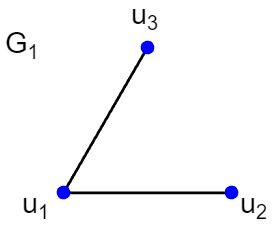
\includegraphics[width=0.9\linewidth]{Ejemplo_1/Ejemplo1_G1.jpg}
            \end{minipage} \hspace{0.1\linewidth}
            \begin{minipage}[h]{0.3\linewidth}
                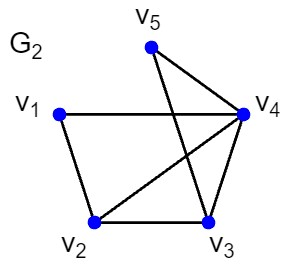
\includegraphics[width=0.9\linewidth]{Ejemplo_1/Ejemplo1_G2.jpg}
            \end{minipage}
        \end{center} \vspace{3mm}

        \begin{enumerate}[1.]
            \item Obtener el grado máximo y mínimo de cada gráfica. En este caso, $ \delta(G_1) = 1, \delta(G_2) = 2 $, \mbox{$ \Delta(G_1) = 2 $} y $ \Delta(G_2) = 4 $. \vspace{3mm}
            \item Elaborar dos tablas donde la primer fila esté conformada por los grados anteriormente obtenidos como se muestra a continuación: \vspace{3mm}
            
            \begin{center}
                \begin{minipage}[h]{0.3\linewidth}
                    \begin{tcolorbox}[title empty, center, colframe = black!99!white, colback = white, sharp corners, hbox, left = -0.9mm, right = -0.9mm, top = -0.9mm, bottom = -0.9mm]
                        \begin{tabular}{c|c}
                            \rowcolor{gray!36!white} 
                            $ \delta(G_1) = 1 $ & $ \Delta(G_2) = 4 $ 
                        \end{tabular}
                    \end{tcolorbox}
                \end{minipage}
                \begin{minipage}[h]{0.3\linewidth}
                    \begin{tcolorbox}[title empty, center, colframe = black!99!white, colback = white, sharp corners, hbox, left = -0.9mm, right = -0.9mm, top = -0.9mm, bottom = -0.9mm]
                        \begin{tabular}{c|c}
                            \rowcolor{gray!36!white} 
                            $ \Delta(G_1) = 2 $ & $ \delta(G_2) = 2 $
                        \end{tabular}
                    \end{tcolorbox}
                \end{minipage}
            \end{center} \vspace{3mm}
            
            \item En las columnas de las tablas que corresponden a los grados máximos de cada gráfica, se coloca el número de la celda anterior disminuido en uno. Mientras que las columnas que corresponden a los grados mínimos se coloca el número de la celda anterior aumentado en uno. Este procedimiento termina hasta que en las columnas del grado mínimo se llegue al grado máximo de la gráfica que corresponda, o en las columnas del grado mínimo se obtenga un cero. \vspace{3mm}
            
            \begin{center}
                \begin{minipage}[h]{0.3\linewidth}
                    \begin{tcolorbox}[title empty, center, colframe = black!99!white, colback = white, sharp corners, hbox, nobeforeafter, left = -0.9mm, right = -0.9mm, top = -0.9mm, bottom = -0.9mm]
                        \begin{tabular}{c|c}
                            \rowcolor{gray!36!white} 
                            $ \delta(G_1) = 1 $ & $ \Delta(G_2) = 4 $ \\ \hline\hline
                            $ 2 $               & $ 3 $ 
                        \end{tabular}
                    \end{tcolorbox}
                \end{minipage}
                \begin{minipage}[h]{0.3\linewidth}
                    \begin{tcolorbox}[title empty, center, colframe = black!99!white, colback = white, sharp corners, hbox, nobeforeafter, left = -0.9mm, right = -0.9mm, top = -0.9mm, bottom = -0.9mm]
                        \begin{tabular}{c|c}
                            \rowcolor{gray!36!white} 
                            $ \Delta(G_1) = 2 $ & $ \delta(G_2) = 2 $ \\ \hline\hline
                            $ 1 $               & $ 3 $ \\ \hline
                            $ 0 $               & $ 4 $
                        \end{tabular}
                    \end{tcolorbox}
                \end{minipage}
            \end{center} \vspace{3mm}

            \item Por último, se dibujan los vértices de ambas gráficas y se hacen adyacentes aquellos que tengan el grado indicado en cada fila, en su respectiva gráfica. \vspace{2mm}
            
            \begin{center}
                $ G_1 \gradial G_2 $

                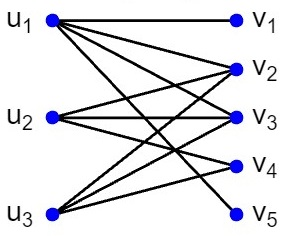
\includegraphics[width=0.3\linewidth]{Ejemplo_1/Ejemplo1_Gg.jpg}
            \end{center}
        \end{enumerate}
    \end{ejemplo}

    Por cómo se definió la gráfica gradial, es claro que ningún par de vértices de cada una de las dos gráficas que la definen son adyacentes entre sí. Esto da lugar a la siguiente proposición.

    \begin{proposicion}[beforeafter skip = 4mm]{}{Gg_bipartita}
        Si $ G_1 $ y $ G_2 $ son gráficas, entonces $ G_1 \gradial G_2 $ es bipartita. 

        \tcblower

        \textbf{Demostración.} \vspace{3mm}

        \begin{list}{\bfseries Afirmación.}{ \addtolength{\itemindent}{-5mm}%
            \addtolength{\labelsep}{0mm}%
            \addtolength{\leftmargin}{-5mm}% 
            \addtolength{\labelwidth}{-1cm} }
            \item $ \left\lbrace \textnormal{V}(G_1), \textnormal{V}(G_2) \right\rbrace $ es una partición de $ \textnormal{V}(G_1 \gradial G_2) $. \vspace{2mm}
            
            \begin{itemize}
                \item $ \textnormal{V}(G_1) $ y $ \textnormal{V}(G_2) $ son no vacíos, por definición de gráfica. 
                \item $ \textnormal{V}(G_1) \cap \textnormal{V}(G_2) \neq \emptyset $ por la definición de gráfica gradial.
                \item $ \textnormal{V}(G_1) \cup \textnormal{V}(G_2) = \textnormal{V}(G_1 \gradial G_2) $ por la definición de gráfica gradial.
            \end{itemize} \vspace{2mm}

            De esta forma, $ \left\lbrace \textnormal{V}(G_1), \textnormal{V}(G_2) \right\rbrace $ es una partición de $ \textnormal{V}(G_1 \gradial G_2) $. 
        \end{list} \vspace{2mm}

        Luego, para $ uv \in \textnormal{A}(G_1 \gradial G_2) $ se tiene que $ u \in \textnormal{V}(G_1) $ y $ v \in \textnormal{V}(G_2) $ ó, $ v \in \textnormal{V}(G_2) $ y $ u \in \textnormal{V}(G_2) $, por definición de gráfica gradial. \vspace{2mm}

        Por lo tanto, $ G_1 \gradial G_2 $ es bipartita.
    \end{proposicion}

    Ya que la gráfica gradial es bipartita se tiene que su número cromático es 2, por lo que hablar de coloración en esta gráfica no es relevante. Por lo tanto, este tema no se tratará.

    \begin{proposicion}[breakable, pad at break = 4mm, beforeafter skip = 4mm]{}{conmutatividad}
        Si $ G_1 $ y $ G_2 $ son gráficas, entonces $ G_1 \gradial G_2 = G_2 \gradial G_1 $.
        
        \tcblower

        \textbf{Demostración.} \vspace{3mm}

        Por definición de gráfica gradial, se da que $ \textnormal{V}(G_1 \gradial G_2) = \textnormal{V}(G_1) \cup \textnormal{V}(G_2) = \textnormal{V}(G_2) \cup \textnormal{V}(G_1) = \textnormal{V}(G_2 \gradial G_1) $. Luego,
        \begin{align*}
            \textnormal{A}(G_1 \gradial G_2) =& \, \bigl\{ uv \mid u \in \textnormal{V}(G_1), \, v \in \textnormal{V}(G_2), \textnormal{ gr}_{G_1}(u) + \textnormal{gr}_{G_2}(v) = \delta(G_1) + \Delta(G_2) \bigr\} \, \cup \\
            & \, \bigl\{ uv \mid u \in \textnormal{V}(G_2), \, v \in \textnormal{V}(G_1), \textnormal{ gr}_{G_2}(u) + \textnormal{gr}_{G_1}(v) = \delta(G_2) + \Delta(G_1) \bigr\} \\
            =& \, \bigl\{ uv \mid u \in \textnormal{V}(G_2), \, v \in \textnormal{V}(G_1), \textnormal{ gr}_{G_2}(u) + \textnormal{gr}_{G_1}(v) = \delta(G_2) + \Delta(G_1) \bigr\} \, \cup \\
            & \, \bigl\{ uv \mid u \in \textnormal{V}(G_1), \, v \in \textnormal{V}(G_2), \textnormal{ gr}_{G_1}(u) + \textnormal{gr}_{G_2}(v) = \delta(G_1) + \Delta(G_2) \bigr\} \\
            =& \, \textnormal{A}(G_2 \gradial G_1)
        \end{align*}
        Por lo tanto, $ G_1 \gradial G_2 = G_2 \gradial G_1 $.
    \end{proposicion}

    \begin{ejemplo}[beforeafter skip = 4mm]{}{conmutatividad}
        Sean $ G_1 $ y $ G_2 $ gráficas, como se muestran abajo, y obteniendo su gráfica gradial.

        \begin{center}
            \begin{minipage}[h]{0.6\linewidth}
                \begin{minipage}[h]{0.45\linewidth}
                    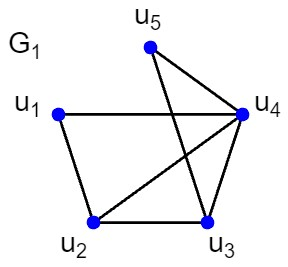
\includegraphics[width=0.9\linewidth]{Ejemplo_2/Ejemplo2_G1.jpg}
                \end{minipage} 
                \begin{minipage}[h]{0.45\linewidth}
                    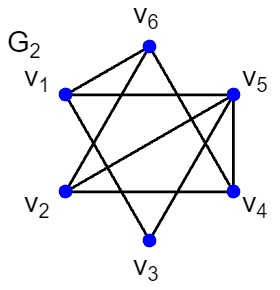
\includegraphics[width=0.9\linewidth]{Ejemplo_2/Ejemplo2_G2.jpg}
                \end{minipage} 
        
                \begin{minipage}[h]{0.45\linewidth}
                    \begin{tcolorbox}[title empty, colframe = black!99!white, colback = white, sharp corners, hbox, nobeforeafter, left = -0.9mm, right = -0.9mm, top = -0.9mm, bottom = -0.9mm]
                        \begin{tabular}{c|c}
                            \rowcolor{gray!36!white} 
                            $ \delta(G_1) = 2 $ & $ \Delta(G_2) = 4 $ \\ \hline\hline
                            $ 3 $               & $ 3 $ \\ \hline
                            $ 4 $               & $ 2 $
                        \end{tabular}
                    \end{tcolorbox}
                \end{minipage}
                \begin{minipage}[h]{0.45\linewidth}
                    \begin{tcolorbox}[title empty, colframe = black!99!white, colback = white, sharp corners, hbox, nobeforeafter, left = -0.9mm, right = -0.9mm, top = -0.9mm, bottom = -0.9mm]
                        \begin{tabular}{c|c}
                            \rowcolor{gray!36!white} 
                            $ \Delta(G_1) = 4 $ & $ \delta(G_2) = 2 $ \\ \hline\hline
                            $ 3 $               & $ 3 $ \\ \hline
                            $ 2 $               & $ 4 $
                        \end{tabular}
                    \end{tcolorbox}
                \end{minipage}
            \end{minipage}
            \begin{minipage}[h]{0.25\linewidth}
                \centering

                $ G_1 \gradial G_2 $

                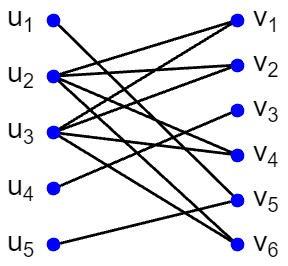
\includegraphics[width = 1\linewidth]{Ejemplo_2/Ejemplo2_Gg.jpg}
            \end{minipage}
        \end{center} \vspace{3mm}

        Si se construye la gráfica $ G_2 \gradial G_1 $, lo único que cambia es el orden de las columnas de las tablas de arriba, las adyacencias siguen siendo las mismas en cualquiera de las dos gráficas gradiales.
    \end{ejemplo}

    En los próximos enunciados se pueden atribuir propiedades concretas a las gráficas que definen la gráfica gradial. Debido a la Proposición \eqref{prop:conmutatividad}, estas propiedades se le pueden atribuir a las gráficas de forma indistinta.

    \textbf{Observación.} Debido a que toda gráfica siempre tiene vértices de grado mínimo o máximo, la gráfica gradial siempre tendrá al menos una arista, cuyos extremos son estos vértices. De esta manera, \mbox{$ \textnormal{A}(G_1 \gradial G_2) \neq \emptyset $}, para cualesquiera dos gráficas $ G_1 $ y $ G_2 $.

    \begin{teorema}[breakable, pad at break = 4mm, beforeafter skip = 4mm]{}{subgrafica_bipartita_completa}
        Sean $ G_1 $ y $ G_2 $ gráficas tal que $ G_1 $ es $ r $-regular. Si $ V' = \left\lbrace v \in \textnormal{V}(G_2) \mid \textnormal{gr}(v) = \delta(G_2) \textnormal{ ó gr}(v) = \Delta(G_2) \right\rbrace $, entonces \vspace{3mm}
        
        \begin{enumerate}
            \item la subgráfica inducida de $ G_1 \gradial G_2 $ por $ \textnormal{V}(G_1) \cup V' $ es bipartita completa.
            \item Todo $ v \in \textnormal{V}(G_2) \setminus V' $ es aislado.
        \end{enumerate}

        \tcblower

        \textbf{Demostración.} \vspace{3mm}

        \begin{enumerate}
            \item Sea $ H = \left\langle \textnormal{V}(G_1) \cup V' \right\rangle_{G_1 \! \gradial \! G_2} $, se tiene que $ \bigl\{ \textnormal{V}(G_1), V' \bigr\} $ es una partición de $ \textnormal{V}(G_1) \cup V' $, pues $ V' \neq \emptyset $, $ \textnormal{V}(G_1) \cap V' \subseteq \textnormal{V}(G_1) \cap \textnormal{V}(G_2) = \emptyset $ y $ \textnormal{V}(G_1) \cup V' = \textnormal{V}(H) $, por ser inducida. \vspace{2mm}

            Después, sea $ uv \in \textnormal{A}(H) $, por definición de gráfica gradial, $ u \in \textnormal{V}(G_1) $ y $ v \in \textnormal{V}' \subseteq \textnormal{V}(G_2) $, ó $ v \in \textnormal{V}(G_1) $ y $ v \in \textnormal{V}' \subseteq \textnormal{V}(G_2) $. Así, $ H $ es bipartita. \vspace{2mm}
    
            Ahora, sean $ w \in \textnormal{V}(G_1) $ y $ x \in \textnormal{V}' $. Como $ G_1 $ es $ r $-regular, se da que $ \Delta(G_1) = r = \delta(G_1) = \textnormal{gr}_{G_1}(w) $. Y ya que $ x \in \textnormal{V}' $ se tiene que $ w \, \textnormal{ady}_H \, x $, puesto que \vspace{2mm}
            
            $ \textnormal{gr}_{G_1}(w) + \textnormal{gr}_{G_2}(x) = r + \Delta(G_2) = \delta(G_1) + \Delta(G_2) $ \; o \; $ \textnormal{gr}_{G_1}(w) + \textnormal{gr}_{G_2}(x) = \delta(G_2) + r = \delta(G_2) + \Delta(G_1) $ \vspace{2mm}
            
            (no hay más posibilidades, pues $ G_1 $ es $ r $-regular y los vértices de \textnormal{V}' son aquellos cuyo grado es máximo o mínimo). \vspace{2mm}
    
            Por lo tanto, $ H $ es una gráfica bipartita completa. \vspace{2mm}

            \item Sea $ v \in \textnormal{V}(G_2) \setminus V' $ existen $ i, j \in \left\lbrace 1, 2, \ldots, \Delta(G_2) - 1 \right\rbrace $ tales que $ \textnormal{gr}_{G_2}(v) = \delta(G_2) + i = \Delta(G_2) - j $ ($ i, j $ son distintos de cero y de $ \Delta(G_2) $, pues $ v \notin V' $). Sea $ u \in \textnormal{V}(G_1) $ se da que $ \textnormal{gr}_{G_1}(u) = r $, por lo que $ u $ no es adyacente a $ v $, ya que de lo contrario, $ \textnormal{gr}_{G_1}(u) = \Delta(G_1) - i = r - i $ o $ \textnormal{gr}_{G_1}(u) = \delta(G_1) + j = r + j $, lo cual no puede ser.
            
            De esta forma, como $ \forall v \in \textnormal{V}(G_2) \setminus V' $, $ v $ no es adyacente a ningún otro vértice, se obtiene que $ v $ es un vértice aislado.
        \end{enumerate} 
    \end{teorema}

    \begin{ejemplo}[beforeafter skip = 4mm]{}{subgrafica_bipartita_completa}
        Sean $ G_1 $ una gráfica $ 4 $-regular y $ G_2 $ una gráfica, como se muestran a continuación. Construyendo su gráfica gradial:

        \begin{center}
            \begin{minipage}[h]{0.6\linewidth}
                \begin{minipage}[h]{0.45\linewidth}
                    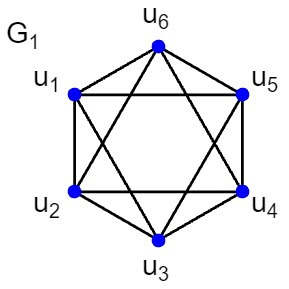
\includegraphics[width=0.9\linewidth]{Ejemplo_3/Ejemplo3_G1.jpg}
                \end{minipage} 
                \begin{minipage}[h]{0.45\linewidth}
                    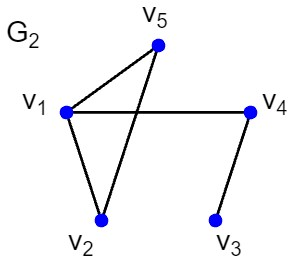
\includegraphics[width=0.9\linewidth]{Ejemplo_3/Ejemplo3_G2.jpg}
                \end{minipage} 
    
                \begin{minipage}[h]{0.45\linewidth}
                    \begin{tcolorbox}[title empty, colframe = black!99!white, colback = white, sharp corners, hbox, nobeforeafter, left = -0.9mm, right = -0.9mm, top = -0.9mm, bottom = -0.9mm]
                        \begin{tabular}{c|c}
                            \rowcolor{gray!36!white} 
                            $ \delta(G_1) = 4 $ & $ \Delta(G_2) = 3 $
                        \end{tabular}
                    \end{tcolorbox}
                \end{minipage}
                \begin{minipage}[h]{0.45\linewidth}
                    \begin{tcolorbox}[title empty, colframe = black!99!white, colback = white, sharp corners, hbox, nobeforeafter, left = -0.9mm, right = -0.9mm, top = -0.9mm, bottom = -0.9mm]
                        \begin{tabular}{c|c}
                            \rowcolor{gray!36!white} 
                            $ \Delta(G_1) = 4 $ & $ \delta(G_2) = 1 $
                        \end{tabular}
                    \end{tcolorbox}
                \end{minipage}
            \end{minipage}
            \begin{minipage}[h]{0.25\linewidth}
                \centering
                
                $ G_1 \gradial G_2 $

                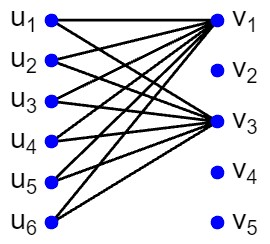
\includegraphics[width = 1\linewidth]{Ejemplo_3/Ejemplo3_Gg.jpg}
            \end{minipage}
        \end{center} \vspace{3mm}

        Como se puede observar, la subgráfica inducida por $ \textnormal{V}(G_1) \cup \lbrace v_1 \rbrace $ de la gráfica gradial es bipartita completa.
    \end{ejemplo}

    En base al ejemplo anterior, es posible deducir que si una gráfica es regular y la otra solo tiene vértices de a lo más dos grados distintos, la gráfica gradial de estas es bipartita completa.

    \begin{corolario}[beforeafter skip = 4mm]{}{maxmin_bipartita_completa}
        Sean $ G_1 $ y $ G_2 $ gráficas. Si $ G_1 $ es $ r $-regular y para todo $ v \in \textnormal{V}(G_2) $ se da que gr$(v) = \delta(G_2) $ ó gr$(v) = \Delta(G_2) $, entonces $ G_1 \gradial G_2 $ es bipartita completa.

        \tcblower

        \textbf{Demostración.} \vspace{3mm}

        Ya que $ \bigl\{ v \in \textnormal{V}(G_2) \mid \textnormal{gr}_{G_2}(v) = \delta(G_2) \textnormal{ ó gr}_{G_2}(v) = \Delta(G_2) \bigr\} = \textnormal{V}(G_2) $, por hipótesis. Por el inciso \textsc{I} del Teorema \eqref{teo:subgrafica_bipartita_completa}, se tiene que $ G_1 \gradial G_2 $ es bipartita completa.
    \end{corolario}

    \begin{corolario}[beforeafter skip = 4mm]{}{regulares_completa}
        Si $ G_1 $ y $ G_2 $ son gráficas $ r $-regular y $ s $-regular, respectivamente, entonces $ G_1 \gradial G_2 $ es bipartita completa.

        \tcblower

        \textbf{Demostración.} \vspace{3mm}

        Debido a que $ \textnormal{gr}_{G_2}(v) = s, \forall v \in \textnormal{V}(G_2) $, se da que $ \Delta(G_2) = s = \delta(G_2) = \textnormal{gr}_{G_2}(v) \; \forall v \in \textnormal{V}(G_2) $, De esta forma, por el Teorema \eqref{teo:subgrafica_bipartita_completa}, $ G_1 \gradial G_2 $ es bipartita completa.
    \end{corolario}

    \textbf{Observaciones.}

    \begin{enumerate}
        \item $ K_n \gradial K_m $ es bipartita completa $ \forall n, m \in \mathbb{N} $, pues $ K_n $ y $ K_m $ son $ (n-1) $-regular y $ (m-1) $-regular, respectivamente.
        \item $ C_n \gradial C_m $ es bipartita completa $ \forall n, m \in \mathbb{N} $, pues $ C_n $ y $ C_m $ son gráficas $ 2 $-regular.
    \end{enumerate} \vspace{1mm}

    Ahora bien, si $ G_1 $ y $ G_2 $ son gráficas tales que $ \delta(G_1) + \Delta(G_2) = \delta(G_2) + \Delta(G_1) $ entonces 
    \begin{align*}
        \hspace{-7mm} \textnormal{A}(G_1 \gradial G_2) &= \bigl\{ uv \mid u \in \textnormal{V}(G_1), \, v \in \textnormal{V}(G_2), \textnormal{ gr}_{G_1}(u) + \textnormal{gr}_{G_2}(v) = \delta(G_1) + \Delta(G_2) \bigr\} \\
        &= \bigl\{ uv \mid u \in \textnormal{V}(G_2), \, v \in \textnormal{V}(G_1), \textnormal{ gr}_{G_2}(u) + \textnormal{gr}_{G_1}(v) = \delta(G_2) + \Delta(G_1) \bigr\}
    \end{align*}
    De esta manera, si hay dos gráficas que cumplan lo anterior solo es necesario seguir el procedimiento del Ejemplo \eqref{ejem:procedimiento_construccion_Gg}, para construir la gráfica de gradial de ambas gráficas, pero con solo una de las dos tablas.

    \begin{ejemplo}[beforeafter skip = 4mm]{}{igualdad_sumas}
        Sean $ G_1 $ y $ G_2 $ gráficas, como se muestran enseguida. Ya que $ \delta(G_1) = 2, \Delta(G_2) = 4, \delta(G_2) = 2 $ y $ \Delta(G_1) = 4 $. Se tiene que $ \delta(G_1) + \Delta(G_2) = \delta(G_2) + \Delta(G_1) $. Luego, construyendo su gráfica gradial: \vspace{2mm}

        \begin{center}
            \begin{minipage}[h]{0.6\linewidth}
                \begin{minipage}[h]{0.45\linewidth}
                    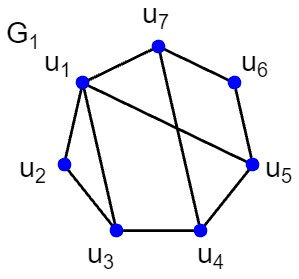
\includegraphics[width=0.9\linewidth]{Ejemplo_4/Ejemplo4_G1.jpg}
                \end{minipage} 
                \begin{minipage}[h]{0.45\linewidth}
                    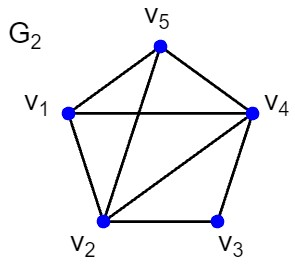
\includegraphics[width=0.9\linewidth]{Ejemplo_4/Ejemplo4_G2.jpg}
                \end{minipage} 
    
                \begin{minipage}[h]{0.45\linewidth}
                    \begin{tcolorbox}[title empty, colframe = black!99!white, colback = white, sharp corners, hbox, nobeforeafter, left = -0.9mm, right = -0.9mm, top = -0.9mm, bottom = -0.9mm]
                        \begin{tabular}{c|c}
                            \rowcolor{gray!36!white} 
                            $ \delta(G_1) = 2 $ & $ \Delta(G_2) = 4 $ \\ \hline \hline
                            $ 3 $               & $ 3 $ \\ \hline
                            $ 4 $               & $ 2 $
                        \end{tabular}
                    \end{tcolorbox}
                \end{minipage}
                \begin{minipage}[h]{0.45\linewidth}
                    \begin{tcolorbox}[title empty, colframe = black!99!white, colback = white, sharp corners, hbox, nobeforeafter, left = -0.9mm, right = -0.9mm, top = -0.9mm, bottom = -0.9mm]
                        \begin{tabular}{c|c}
                            \rowcolor{gray!36!white} 
                            $ \Delta(G_1) = 4 $ & $ \delta(G_2) = 2 $ \\ \hline \hline
                            $ 3 $               & $ 3 $ \\ \hline
                            $ 2 $               & $ 4 $
                        \end{tabular}
                    \end{tcolorbox}
                \end{minipage}
            \end{minipage}
            \begin{minipage}[h]{0.25\linewidth}
                \centering
                
                $ G_1 \gradial G_2 $

                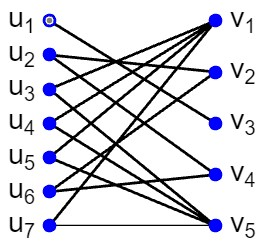
\includegraphics[width = 1\linewidth]{Ejemplo_4/Ejemplo4_Gg.jpg}
            \end{minipage}
        \end{center} \vspace{3mm}

        Las tablas tienen los mismos valores en sus respectivas filas, por lo cual solo es necesario hacer una para construir la gráfica gradial.
    \end{ejemplo}

    \begin{teorema}[breakable, pad at break = 4mm, beforeafter skip = 4mm]{}{Gg_igual_complementos}
        Si $ G_1 $ y $ G_2 $ son gráficas, entonces $ G_1 \gradial G_2 = G_1^C \gradial G_2^C $.

        \tcblower

        \textbf{Demostración.} \vspace{3mm}

        Por definición de gráfica gradial y del complemento de una gráfica, se da que $ \textnormal{V}(G_1 \gradial G_2) = \textnormal{V}(G_1) \cup \textnormal{V}(G_2) = \textnormal{V}\left( G_1^C \right) \cup \textnormal{V}\left( G_2^C \right) = \textnormal{V}\left( G_1^C \gradial G_2^C \right) $. \vspace{2mm}

        Ahora, sean $ p_1 = \left\lvert \textnormal{V}(G_1) \right\rvert $ y $ p_2 = \left\lvert \textnormal{V}(G_2) \right\rvert $. Como para cada $ u \in \textnormal{V}(G_1) $ se da que $ \textnormal{gr}_{G_1^C}(u) = p_1 - 1 - \textnormal{gr}_{G_1}(u) $, en particular, $ \Delta\left( G_1^C \right) = p_1 - 1 - \delta(G_1) $ y $ \delta\left( G_1^C \right) = p_1 - 1 - \Delta(G_1) $. De forma análoga, para cada $ v \in \textnormal{V}(G_2) $ se tiene que $ \textnormal{gr}_{G_2^C}(v) = p_2 - 1 - \textnormal{gr}_{G_2}(v) $, en particular, $ \Delta\left( G_2^C \right) = p_2 - 1 - \delta(G_2) $ y $ \delta\left( G_2^C \right) = p_2 - 1 - \Delta(G_2) $. De esta forma,
        \begin{align*}
            \hspace{-7mm} \textnormal{A}(G_1 \gradial G_2) =& \, \bigl\{ uv \mid u \in \textnormal{V}(G_1), \, v \in \textnormal{V}(G_2), \textnormal{ gr}_{G_1}(u) + \textnormal{gr}_{G_2}(v) = \delta(G_1) + \Delta(G_2) \bigr\} \, \cup \\
            & \, \bigl\{ uv \mid u \in \textnormal{V}(G_2), \, v \in \textnormal{V}(G_1), \textnormal{ gr}_{G_2}(u) + \textnormal{gr}_{G_1}(v) = \delta(G_2) + \Delta(G_1) \bigr\} \\
            =& \, \bigl\{ uv \mid u \in \textnormal{V}(G_1), \, v \in \textnormal{V}(G_2), p_1 - 1 - \textnormal{gr}_{G_1}(u) + p_2 - 1 - \textnormal{gr}_{G_2}(v) = p_1 - 1 - \delta(G_1) + p_2 \bigr. - \\ 
            & \quad 1 - \Delta(G_2) \bigr\} \, \cup \, \bigl\{ uv \mid u \in \textnormal{V}(G_2), \, v \in \textnormal{V}(G_1), p_2 - 1 - \textnormal{gr}_{G_2}(u) + p_1 - 1 - \textnormal{gr}_{G_1}(v) = p_2 - \\
            & \quad \bigl. 1 - \delta(G_2) + p_1 - 1 - \Delta(G_1) \bigr\} \\
            =& \, \left\lbrace uv \mid u \in \textnormal{V}(G_1), \, v \in \textnormal{V}(G_2), \textnormal{ gr}_{G_1^C}(u) + \textnormal{gr}_{G_2^C}(v) = \Delta\left( G_1^C \right) + \delta\left( G_2^C \right) \right\rbrace \, \cup \\
            & \, \left\lbrace uv \mid u \in \textnormal{V}(G_2), \, v \in \textnormal{V}(G_1), \textnormal{ gr}_{G_2^C}(u) + \textnormal{gr}_{G_1^C}(v) = \Delta\left( G_2^C \right) + \delta\left( G_1^C \right) \right\rbrace \\
            =& \, \left\lbrace vu \mid v \in \textnormal{V}(G_1), \, u \in \textnormal{V}(G_2), \textnormal{gr}_{G_1^C}(v) + \textnormal{ gr}_{G_2^C}(u) = \delta\left( G_1^C \right) + \Delta\left( G_2^C \right) \right\rbrace \, \cup \\
            & \, \left\lbrace vu \mid v \in \textnormal{V}(G_2), \, u \in \textnormal{V}(G_1), \textnormal{gr}_{G_2^C}(v) + \textnormal{ gr}_{G_1^C}(u) = \delta\left( G_2^C \right) + \Delta\left( G_1^C \right) \right\rbrace \\
            =& \, \textnormal{A}\left( G_1^C \gradial G_2^C \right)
        \end{align*}
        Por lo tanto, $ G_1 \gradial G_2 = G_2 \gradial G_1 $.
    \end{teorema}

    \begin{ejemplo}[breakable, pad at break = 4mm, beforeafter skip = 4mm]{}{Gg_igual_complementos}
        Sean $ G_1 $ y $ G_2 $ gráficas, como se muestran abajo y construyendo su gráfica gradial: \vspace{2mm}

        \begin{center}
            \begin{minipage}[h]{0.6\linewidth}
                \begin{minipage}[h]{0.45\linewidth}
                    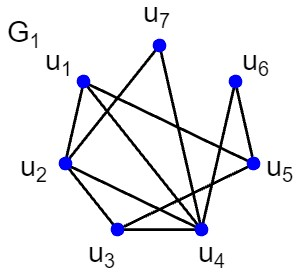
\includegraphics[width=0.9\linewidth]{Ejemplo_5/Ejemplo5_G1.jpg}
                \end{minipage} 
                \begin{minipage}[h]{0.45\linewidth}
                    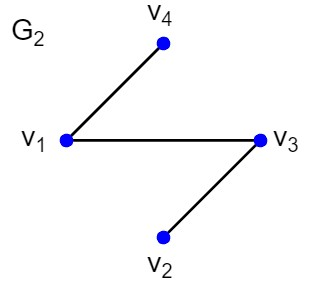
\includegraphics[width=0.9\linewidth]{Ejemplo_5/Ejemplo5_G2.jpg}
                \end{minipage} 
    
                \begin{minipage}[h]{0.45\linewidth}
                    \begin{tcolorbox}[title empty, colframe = black!99!white, colback = white, sharp corners, hbox, nobeforeafter, left = -0.9mm, right = -0.9mm, top = -0.9mm, bottom = -0.9mm]
                        \begin{tabular}{c|c}
                            \rowcolor{gray!36!white} 
                            $ \delta(G_1) = 2 $ & $ \Delta(G_2) = 2 $ \\ \hline \hline
                            $ 3 $               & $ 1 $ \\ \hline
                            $ 4 $               & $ 0 $
                        \end{tabular}
                    \end{tcolorbox}
                \end{minipage}
                \begin{minipage}[h]{0.45\linewidth}
                    \begin{tcolorbox}[title empty, colframe = black!99!white, colback = white, sharp corners, hbox, nobeforeafter, left = -0.9mm, right = -0.9mm, top = -0.9mm, bottom = -0.9mm]
                        \begin{tabular}{c|c}
                            \rowcolor{gray!36!white} 
                            $ \Delta(G_1) = 5 $ & $ \delta(G_2) = 1 $ \\ \hline \hline
                            $ 4 $               & $ 2 $
                        \end{tabular}
                    \end{tcolorbox}
                \end{minipage}
            \end{minipage}
            \begin{minipage}[h]{0.25\linewidth}
                \centering
                
                $ G_1 \gradial G_2 $

                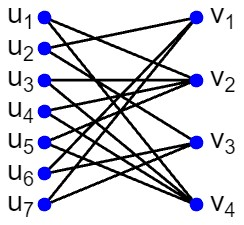
\includegraphics[width = 1\linewidth]{Ejemplo_5/Ejemplo5_Gg.jpg}
            \end{minipage}
        \end{center} \vspace{3mm}

        Ahora, se obtiene la gráfica gradial de sus complementos. \vspace{2mm}

        \begin{center}
            \begin{minipage}[h]{0.6\linewidth}
                \begin{minipage}[h]{0.45\linewidth}
                    $ G_1^C $

                    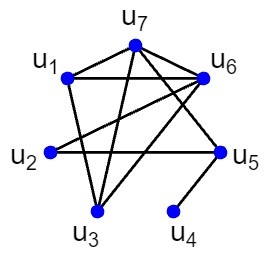
\includegraphics[width=0.9\linewidth]{Ejemplo_5/Ejemplo5_G1C.jpg}
                \end{minipage} 
                \begin{minipage}[h]{0.45\linewidth}
                    $ G_2^C $

                    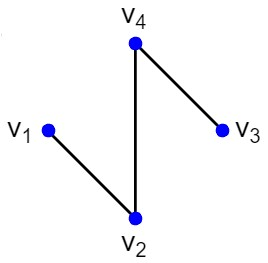
\includegraphics[width=0.9\linewidth]{Ejemplo_5/Ejemplo5_G2C.jpg}
                \end{minipage} 
    
                \begin{minipage}[h]{0.45\linewidth}
                    \begin{tcolorbox}[title empty, colframe = black!99!white, colback = white, sharp corners, hbox, nobeforeafter, left = -0.9mm, right = -0.9mm, top = -0.9mm, bottom = -0.9mm]
                        \begin{tabular}{c|c}
                            \rowcolor{gray!36!white} 
                            $ \delta(G_1) = 1 $ & $ \Delta(G_2) = 2 $ \\ \hline \hline
                            $ 2 $               & $ 1 $ \\ \hline
                            $ 3 $               & $ 0 $
                        \end{tabular}
                    \end{tcolorbox}
                \end{minipage}
                \begin{minipage}[h]{0.45\linewidth}
                    \begin{tcolorbox}[title empty, colframe = black!99!white, colback = white, sharp corners, hbox, nobeforeafter, left = -0.9mm, right = -0.9mm, top = -0.9mm, bottom = -0.9mm]
                        \begin{tabular}{c|c}
                            \rowcolor{gray!36!white} 
                            $ \Delta(G_1) = 4 $ & $ \delta(G_2) = 1 $ \\ \hline \hline
                            $ 3 $               & $ 2 $
                        \end{tabular}
                    \end{tcolorbox}
                \end{minipage}
            \end{minipage}
            \begin{minipage}[h]{0.25\linewidth}
                \centering
                
                $ G_1^C \gradial G_2^C $

                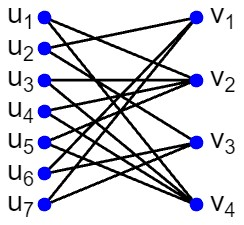
\includegraphics[width = 1\linewidth]{Ejemplo_5/Ejemplo5_Gg.jpg}
            \end{minipage}
        \end{center} \vspace{3mm}

        Las gráficas gradiales son iguales.
    \end{ejemplo}

    \begin{teorema}[beforeafter skip = 4mm]{}{trayectoria_minima}
        Sean $ G_1 $ y $ G_2 $ gráficas. Si para $ u,v \in \textnormal{V}(G_1) $ existe una $ uv $-trayectoria en $ G_1 \gradial G_2 $ entonces existe una $ uv $-trayectoria $ T $ en $ G_1 \gradial G_2 $ de longitud 2, con $ T = (u,w,v) $ donde $ w \in \textnormal{V}(G_2) $.
        
        \tcblower

        \textbf{Demostración.} \vspace{3mm}

        Sea $ T = \left( u = w_0, w_1, \ldots, w_n = v \right) $ una $ uv $-trayectoria en $ G_1 \gradial G_2 $ de longitud mínima. Suponiendo que $ l(T) \neq 2 $, ya que $ G_1 \gradial G_2 $ es bipartita con partición $ \left\lbrace \textnormal{V}(G_1), \textnormal{V}(G_2) \right\rbrace $, se tiene que $ l(T) $ es par, pues de lo contrario, se tendría que $ v \in \textnormal{V}(G_2) $, lo cual no puede ser. Así, $ l (T) \geq 4 $, por lo que se puede asegurar que cuanto menos existen $ w_1, w_3 \in \textnormal{V}(G_2) $ y $ w_2 \in \textnormal{V}(G_1) $ vértices de $ T $. \vspace{2mm}

        Luego, sea $ i \in \left\lbrace 0, 1, \ldots, \Delta(G_1) \right\rbrace $ tal que $ \textnormal{gr}_{G_1}(u) = \Delta(G_1) - i $. Suponiendo, sin pérdida de generalidad, que pasa lo siguiente: Como $ uw_1 \in \textnormal{A}(G_1 \gradial G_2) $ se da que $ \textnormal{gr}_{G_2}(w_1) = \delta(G_2) + i $, luego, ya que $ w_1w_2 \in \textnormal{A}(G_1 \gradial G_2) $, se obtiene que $ \textnormal{gr}_{G_1}(w_2) = \Delta(G_1) - i $ y puesto que $ w_2w_3 \in \textnormal{A}(G_1 \gradial G_2) $ se tiene que $ \textnormal{gr}_{G_2}(w_3) = \delta(G_2) + i $. De esta forma, $ uw_3 \in \textnormal{A}(G_1 \gradial G_2) $, por definición. \vspace{2mm}

        Después, sea $ T' = \left( u = w_0, w_3, \ldots, w_n = v \right) $ se da que $ l(T) > l(T') $, lo cual es una contradicción a que $ T $ es de longitud mínima. Por lo tanto, $ l(T) = 2 $ y $ T = (u,w_1,v) $ con $ w_1 \in \textnormal{V}(G_2) $.
    \end{teorema}

    \begin{teorema}[breakable, pad at break = 4mm, beforeafter skip = 4mm]{}{disconexidad_igualdad_gradial}
        Sean $ G_1 $ y $ G_2 $ gráficas. Si $ \delta(G_1) = \delta(G_2) < \Delta(G_1) = \Delta(G_2) $ entonces $ G_1 \gradial G_2 $ es disconexa.
        
        \tcblower

        \textbf{Demostración.} \vspace{3mm}

        Sean $ u,v \in \textnormal{V}(G_1) $ tales que $ \textnormal{gr}_{G_1}(u) \neq \textnormal{gr}_{G_1}(v) $ (esto se puede asegurar pues $ \delta(G_1) < \Delta(G_1) $, por hipótesis). Suponiendo que existe una $ uv $-trayectoria en $ G_1 \gradial G_2 $, por el Teorema \eqref{teo:trayectoria_minima}, se tiene que existe una $ uv $-trayectoria $ T = (u,w,v) $ en $ G_1 \gradial G_2 $, con $ w \in \textnormal{V}(G_2) $. \vspace{2mm}

        Luego, sean $ i, j \in \left\lbrace 0, 1, \ldots, \Delta(G_1) - \delta(G2) \right\rbrace $ tales que $ \textnormal{gr}_{G_1}(u) = \delta(G_1) + i $ y $ \textnormal{gr}_{G_1}(v) = \delta(G_1) + j $. Debido a que $ uw, wv \in \textnormal{A}(G_1 \gradial G_2) $, suponiendo, sin pérdida de generalidad que, $ \textnormal{gr}_{G_2}(w) = \Delta(G_2) - i $ y $ \textnormal{gr}_{G_2}(w) = \Delta(G_2) - j $, por lo cual, $ \Delta(G_2) - i = \Delta(G_2) - j \Longrightarrow i = j $. Así, $ \textnormal{gr}_{G_1}(u) = \delta(G_1) + i = \delta(G_1) + j = \textnormal{gr}_{G_1}(v) $, lo cual contradice que $ u $ y $ v $ tengan distinto grado en $ G_1 $. De esta manera, no existe una $ uv $-trayectoria en $ G_1 \gradial G_2 $. \vspace{2mm}

        Por lo tanto, $ G_1 \gradial G_2 $ es disconexa.
    \end{teorema}

    En el Ejemplo \eqref{ejem:igualdad_sumas}, se visualiza lo del teorema anterior.

    \begin{corolario}[breakable, pad at break = 4mm, beforeafter skip = 4mm]{}{graficas_isomorfas}
        Si $ G_1 $ y $ G_2 $ son gráficas no regulares tales que $ G_1 \cong G_2 $, entonces $ G_1 \gradial G_2 $ es disconexa.

        \tcblower

        \textbf{Demostración.} \vspace{3mm}

        Ya que $ G_1 \cong G_2 $ se tiene que $ \delta(G_1) = \delta(G_2) < \Delta(G_1) = \Delta(G_2) $, puesto que $ G_1 $ y $ G_2 $ no son regulares. Así, por el Teorema \eqref{teo:disconexidad_igualdad_gradial}, $ G_1 \gradial G_2 $ es disconexa.
    \end{corolario}

    \begin{definicion}{}{gradialmente_sucesiva}
        Sea $ G $ una gráfica con $ \left\lbrace \textnormal{gr}(u) \mid u \in \textnormal{V}(G) \right\rbrace = \left\lbrace \delta(G), \delta(G) + 1, \ldots, \Delta(G) - 1, \Delta(G) \right\rbrace $, se dice que \textbf{$ G $ es gradialmente sucesiva}.
    \end{definicion}

    \begin{ejemplo}{}{}
        La gráfica $ G_1 $ del Ejemplo \eqref{ejem:igualdad_sumas}, es gradialmente sucesiva, porque los grados de sus vértices son 2, 3 y 4, los cuales son números consecutivos.
    \end{ejemplo}

    \textbf{Observación.} Sea $ G $ una gráfica. Para cualesquiera $ u, v \in \textnormal{V}(G) $, se define la relación " $ u $ se relaciona con $ v $ " si y solo si $ \textnormal{gr}(u) = \textnormal{gr}(v) $.

    \begin{itemize}
        \item Ya que $ \forall u \in \textnormal{V}(G) $, se da que $ \textnormal{gr}(u) = \textnormal{gr}(u) $ se tiene que " $ u $ se relaciona con $ u $ ".
        \item Si " $ u $ se relaciona con $ v $ " entonces $ \textnormal{gr}(u) = \textnormal{gr}(v) $ si y solo si $ \textnormal{gr}(v) = \textnormal{gr}(u) $, por lo que " $ v $ se relaciona con $ u $ ".
        \item Si " $ u $ se relaciona con $ v $ " y " $ v $ se relaciona con $ w $ ", entonces $ \textnormal{gr}(u) = \textnormal{gr}(v) $ y $ \textnormal{gr}(v) = \textnormal{gr}(w) $, por lo cual, $ \textnormal{gr}(u) = \textnormal{gr}(w) $. De esta manera, " $ u $ se relaciona con $ w $ ".
    \end{itemize}

    Por lo tanto, la relación antes definida es de equivalencia, dando lugar a la siguiente definición.

    \begin{definicion}{}{}
        Sea $ G $ una gráfica. La \textbf{clase $ i $-gradial de $ G $}, se define y denota como \vspace{3mm}

        $ C_G(i) = \left\lbrace u \in \textnormal{V}(G) \mid \textnormal{gr}(u) = i \right\rbrace $ para cada $ i = \delta(G), \delta(G) + 1, \ldots, \Delta(G) $.
    \end{definicion}

    \textbf{Observaciones.}

    \begin{enumerate}[1.]
        \item  Cuando se hable de cualquier clase $ i $-gradial de alguna gráfica, solo se le llamará \textbf{clase gradial}.
        \item Sean $ G_1, G_2 $ gráficas y $ u \in \textnormal{V}(G_1) $ tal que $ \textnormal{gr}_{G_1}(u) = \delta(G_1) + i = \Delta(G_1) - j $ para algunos \\ $ i, j \in \left\lbrace 0, 1, \ldots, \max\left\lbrace \Delta(G_1) - \delta(G_1), \Delta(G_1) \right\rbrace \right\rbrace $. Si $ u \, \textnormal{ady}_{G_1 \! \gradial \! G_2} \, v $, para algún $ v \in \textnormal{V}(G_2) $, entonces $ \textnormal{gr}_{G_2}(v) = \Delta(G_2) - i $ o $ \textnormal{gr}_{G_2}(v) = \delta(G_1) + j $. Además de que todos los vértices que tengan estos grados también serán adyacentes a $ u $ De esta manera, cada $ u \in \textnormal{V}(G_1) $ puede ser adyacente a los vértices de a lo más 2 clases gradiales distintas de $ G_2 $. Esto también se cumple de forma inversa.
    \end{enumerate}

    \begin{teorema}{}{clases_mayores}
        Sean $ G_1 $ y $ G_2 $ gráficas, con $ G_1 $ gradialmente sucesiva y no regular. Si hay $ n $ clases gradiales de $ G_2 $ y $ G_1 $ tiene más de $ 2n $ clases gradiales, entonces $ G_1 \gradial G_2 $ es disconexa.

        \tcblower

        \textbf{Demostración.} \vspace{3mm}

        \begin{list}{\bfseries Caso 1.}{ \addtolength{\itemindent}{-5mm}%
            \addtolength{\labelsep}{0mm}%
            \addtolength{\leftmargin}{-5mm}% 
            \addtolength{\labelwidth}{-1cm} }
            \item Si existe $ v \in \textnormal{V}(G_2) $ tal que $ v $ no es adyacente a algún $ u \in \textnormal{V}(G_1) $, entonces $ G_1 \gradial G_2 $ es disconexa. \vspace{2mm}
            \item Si para cada $ v \in \textnormal{V}(G_2) $ se da que $ v \, \textnormal{ady}_{G_1 \! \gradial \! G_2} \, u $ para algún $ u \in \textnormal{V}(G_1) $, entonces cada vértice de $ G_2 $ es adyacente a los vértices de a lo más 2 clases gradiales de $ G_1 $. De esta manera, los vértices de $ G_2 $ son adyacentes a todos los vértices de hasta $ 2n $ clases gradiales de $ G_1 $, por lo que existe $ j \in \left\lbrace \delta(G_1), \delta(G_1) + 1, \ldots, \Delta(G_2) \right\rbrace $ tal que los vértices de la clase $ j $-gradial de $ G_1 $ no son adyacentes a ningún vértice de $ G_2 $. 

            Por lo tanto, $ G_1 \gradial G_2 $ es disconexa.
        \end{list}
    \end{teorema}

    \begin{proposicion}{}{}
        Sean $ G_1 $ y $ G_2 $ gráficas no regulares. Si hay $ \delta(G_1) + \Delta(G_2) = \delta(G_2) + \Delta(G_1) $ y $ G_1 $ es gradialmente sucesiva, pero $ G_2 $ no lo es, entonces $ G_1 \gradial G_2 $ es disconexa.

        \tcblower

        \textbf{Demostración.} \vspace{3mm}

        Como $ G_2 $ no es gradialmente sucesiva, existe $ i \in \left\lbrace 0, 1, \ldots, \Delta(G_2) \right\rbrace $ tal que $ C_{G_2}(\Delta(G_2) - i) = \emptyset $. Ya que $ \delta(G_1) + \Delta(G_2) = \delta(G_2) + \Delta(G_1) $ se tiene que cualquier vértice de $ G_1 $ es adyacente a los vértices de a lo más una clase gradial de $ G_2 $ y viceversa. De esta forma, para todo $ v \in C_{G_2}(\delta(G_1) + i) \neq \emptyset $, $ v $ es un vértice aislado pues en $ G_2 $ no existe un vértice de grado $ \Delta(G_2) - i $. \vspace{2mm}

        Por lo tanto, $ G_1 \gradial G_2 $ es disconexa.
    \end{proposicion}
    
\end{document}